% !TeX spellcheck = en_US

\chapter{Quantitative Analysis of PET Plastic Debris in Soil via TGA/MS}
\label{ch:tga-ms-method}

\paragraph{Abstract} The use of plastic materials in daily life\marginnote{This chapter is based on: \fullcite{DavidQuantitative2018}.\par See \nameref{ch:author-contributions}, page~\pageref{ch:author-contributions}, for details.}, industry, and agriculture can cause soil pollution with plastic debris down to the micrometer range, namely, microplastics.
The quantitative assessment of plastic debris in soil has been limited so far. Until now, microplastic analyses in soil require laborious sample cleanup and are mostly restricted to qualitative assessments. In this study, we applied \ac{tga-ms} to develop a method for the direct quantitative analysis of \ac{pet} without further sample preparation.
For this, soil samples containing \SI{1.6(2)}{\percent} \ac{Corg} were spiked at \SIrange{2.3}{45.9}{\gram\per\kilo\gram} \ac{pet} plastic debris from recycled bottles. \textsc{dl}-Cysteine was used as an internal standard. Sample mixtures were pyrolyzed with a \SI{5}{\kelvin\per\minute} ramp (\SIrange{40}{1000}{\degreeCelsius}), while sample mass loss and \ac{ms} signal intensities of typical \ac{pet} pyrolysis products were recorded.
We found signal intensities linearly responding to \ac{pet} concentrations. The most promising results were obtained with the internal standard-corrected \ac{pet} pyrolysis product vinylbenzene\slash benzoic acid (\SI{105}{\mz}, adj. $R^2$ = \num{0.987}). The \acp{lod} and \acp{loq} were \SIlist{0.7;17.2}{\gram\per\kilo\gram} \ac{pet}, respectively.
Our results suggest that \ac{tga-ms} can be an easy and viable complement to existing methods such as \ac{ted-gc-ms} or microspectroscopic techniques.

\section{Introduction}

Microplastics are synthetic polymers with typical particle sizes smaller than \SI{5}{\milli\meter} either disintegrated from larger plastic parts or originally produced in particulate form \citep{CincinelliMicroplastic2017}.
Microplastics have been recently recognized as a ubiquitous environmental contaminant in marine and fresh waters, sediments, and organisms \citep{KarlssonScreening2017,RochmanMicroplastics2018}. However, the sources, pathways, and reservoirs of microplastics in terrestrial systems are still hardly known \citep{DrisSynthetic2016}.

Microplastics could be introduced into soil via
\begin{enumerate*}
	\item air transport of non-managed plastic wastes, littering, and street runoff \citep{DrisSynthetic2016,BlasingPlastics2018},
	\item disintegration of agriculture plastics such as mulch films, tarpaulins, tunnels, and pipes \citep{LambertOccurrence2014}, or
	\item application of sewage sludge and reclaimed wastewater containing plastic microbeads or
	fibers \citep{BlasingPlastics2018,ZubrisSynthetic2005}.
\end{enumerate*}
In this respect, the presence of plastic fragments has become an important parameter to describe urban soils and Technosols \citep{RilligMicroplastic2012,NizzettoAre2016}. Particularly in transitional and developing economies, used agricultural plastic mulches and other plastic wastes may be incorporated into the soil of agricultural fields \citep{DuisMicroplastics2016} and household gardens \citep{vanderWalHuertos2011}, where they are likely to become an environmental issue \citep{SintimBiodegradable2017}. Plastic debris is assumed to further accumulate in the soil food web \citep{RilligMicroplastic2012}, to function as sorbent for agrochemicals \citep{RamosPolyethylene2015}, or adversely affect soil organisms \citep{KirsteinDangerous2016}, eventually decreasing soil stability and quality.
Synthetic polyester fibers, namely \ac{pet}, as used in this screening study, have already been found in sewage sludge \citep{ZubrisSynthetic2005} and are continuously introduced into the environment by washing and wearing synthetic textiles \citep{PircEmissions2016}. Agricultural tarpaulins or discarded \ac{pet} bottles are another source of plastic pollution in soil.

In order to assess the content of plastic debris in agricultural soil and adjacent freshwater sediments, analytical assays for the identification and quantification of plastic debris in complex environmental matrices are needed \citep{BlasingPlastics2018}. Microscopic techniques, mainly light microscopy, are currently the most used but pose extraordinarily high requirements on laboratory cleanliness and typically require labor-intensive preconcentration procedures \citep{WoodallUsing2015}. If these requirements are not
met, misinterpretation coming from false positive results is likely \citep{LachenmeierMicroplastic2015}. Microspectroscopic techniques, such as \ac{ftir} spectroscopy with optional \ac{atr} or Raman microspectrometry, represent alternative approaches. The latter may help to fulfill the analytical requirements of distinguishing particles or fibers of synthetic origin from natural matrix structures such as cellulose fibers or silicate particles. \citet{PrimpkeAutomated2017} presented an interesting method for the automated detection of plastic debris on membrane filters using advanced image analysis software. Such techniques have been used for more easily accessible and homogeneous atmospheric or aqueous matrices so far but not for soil \citep{IoakeimidisDegradation2016,FischerIdentification2015,Comnea-StancuIdentification2016}, and they often produce only qualitative results \citep{BlasingPlastics2018} because of interferences from \ac{som} autofluorescence.

Another promising technique may be alkali depolymerization of \ac{pet} and subsequent analysis of depolymerized building blocks bisphenol A and \textit{p}-phthalic acid in sludge, sediments, and mussels via \ac{lc-ms} \citep{WangSimple2017}. However, both bisphenol A and \textit{p}-phthalic acid are not specific for the analysis of one single polymer, extraction from soil may be incomplete, and leaching and mobilization of building block compounds from the polymer backbone into the environment may produce ambiguous results \citep{WangSimple2017}. \citet{ElertComparison2017} achieved recovery rates of about \SI{80}{\percent} \ac{pet} extracted from soil with hexafluoroisopropanol followed by \ac{sec} and reverse-phase \ac{lc}.

In contrast, analytical techniques based on sample pyrolysis have the potential to overcome the aforementioned drawbacks of microscopic and extraction methods in terms of higher specificity, lower sample preparation efforts, and facilitation of semiquantitative to quantitative analyses.
For example, by using Curie point \ac{py-gc-ms}, \ac{pet} quantification in fish required less than \SI{5}{\micro\gram} of substance when combined with prior enzymatic and chemical digestion \citep{FischerSimultaneous2017}.
However, high sand contents made an additional density separation step necessary, which is challenging considering the high density of \ac{pet}. Here, \citet{DumichenAnalysis2015} were the first to successfully apply and validate a quantitative method for \ac{pe} in soil.
The authors established a two-step procedure involving pyrolysis of \ac{pe}-spiked soil via \ac{tga} and capturing of pyrolysis gases followed by \ac{ted-gc-ms}. The same method has also been applied for the determination of \ac{pet}, so far only with qualitative results \citep{DumichenFast2017}.

An alternative to this two-step approach is on-line \ac{tga-ms}, measuring simultaneously the masses of gases evolving during thermal treatment. Thermal treatment can either be oxidation (combustion) or pyrolysis in an inert \ch{Ar} atmosphere. A defined portion of gaseous degradation products are transferred into a quadrupole \ac{ms} via a heated capillary or a capillary\-/less orifice. The mass loss at a specific temperature is then related to the \ac{ms} signal of gaseous pyrolysis products.
Even without chromatographic separation, analytes with the same or similar pyrolysis products as the matrix may be distinguished from each other\sidenote{For instance plastic pyrolysis products from soil pyrolysis products.} according to their distinct decomposition temperatures.

So far, \ac{tga-ms} has been successfully applied for characterizing combustion or pyrolysis products of soils \citep{PallasserSoil2013,EdmondsonBlack2015,TamimiFate2017}, sediments \citep{FindorakovaAssessment2017}, and polymers \citep{PagaczThermal2015,SchindlerNovel2013}. However, complex mixtures of plastic debris and soil have not yet been assessed.
With this proof\-/of\-/principle work, we aimed to evaluate the potential of a capillary \ac{tga-ms} system to qualitatively and quantitatively determine \ac{pet} in a spiked soil without any preseparation of \ac{pet} plastic debris from soil.
We focused on the determination and quantification of characteristic pyrolysis products of \ac{pet} such as benzoic acid and vinyl and alkylbenzenes (\SI{105}{\mz} fragment) and biphenyl (\SI{154}{\mz} fragment) \citep{DumichenFast2017,DimitrovAnalysis2013,DuemichenAssessment2014}; the latter being formed by a radical reaction and intramolecular ring formation \citep{RichterFormation2000,KawaiCharacterization2008}.
The formation of these pyrolysis products can then be related to their specific degradation temperatures as determined by \ac{tga}. \textsc{dl}-Cysteine was used as internal standard for normalizing the present detector signal and ionization state.
By using a capillary \ac{tga-ms}, we wanted to provide an easy-to-use instrumental setup for plastic analysis. Since some studies have discussed the potential of the \ac{tga-ms} capillary to become blocked during polymer measurements \citep{SchindlerNovel2013,DuemichenAssessment2014}, particular attention was paid to monitoring and maintaining a working capillary throughout all our experiments.
In this work, we study the possibilities of using the capillary \ac{tga-ms} device for a quicker and cheaper assessment of plastic debris in soil within the soil matrix and the influences of \ac{som} on the detection limits.

\section{Experimental}

\subsection{Materials}

Cryomilled \ac{pet} dust obtained from mechanical shredding of bottle recyclate\sidenote{PETKA CZ, Brno, Czech Republic.} (\SIrange{0.15}{0.4}{\milli\meter} dominant particle size) was used as the microplastic sample. \Iac{pet} standard\sidenote{\cas{25038-59-9}, PlasticsEurope, Frankfurt, Germany.} and \iac{pet} water bottle sample\sidenote{EDEKA, Hamburg, Germany.} were used to assess \ac{pet} dust quality.
For the preparation of calibration series, a standard loamy sand (\SI{75}{\percent} sand, \SI{16}{\percent} silt, \SI{9}{\percent} clay)\sidenote{LUFA 2.2, \foreignlanguage{ngerman}{Landwirtschaftliche Unter\-suchungs- und Forschungsanstalt}, Speyer, Germany.} with \SI{1.6(2)}{\percent} \ac{Corg} content was used. \textsc{dl}-Cysteine\sidenote{\cas{3374-22-9}, \SI{98}{\percent} purity, Carl Roth, Karlsruhe, Germany.} served as the internal standard for \ac{tga-ms} pyrolysis measurements.

\subsection{Quality Assessment of the \Acs{pet} Dust}

In order to compare the potential difference in the physicochemical properties of the shredded microplastic sample and the \ac{pet} standard, \ac{dsc}\sidenote{Q1000, TA Instruments, New Castle, USA.} was used to determine their melting temperature and melting enthalpy.
The thermal history of \ac{pet} samples was erased with a preheating run from \SIrange[range-phrase = { to }]{40}{310}{\degreeCelsius} followed by a cooling run from \SIrange[range-phrase = { to }]{310}{-20}{\degreeCelsius}.
For the subsequent measurement, the heating run was repeated from \SIrange[range-phrase = { to }]{-20}{310}{\degreeCelsius}. All runs were performed in hermetically sealed pans\sidenote{TZero, TA Instruments, New Castle, USA.} under a \SI{50}{\milli\liter\per\minute} \ch{N2} flow and a thermal ramp of \SI{+-10}{\kelvin\per\minute}. All \ac{dsc} analyses were performed in triplicate.

\subsection{Preparation of Spiked Soil Samples}

Two calibration series were prepared, each in duplicate. For both experiments, a microscale\sidenote{Sartorius SE 02-OCE, Göttingen, Germany.} and \SI{85}{\micro\liter} alumina \ac{tga} crucibles\sidenote{Netzsch, Selb, Germany.\label{sn:netzsch}} were used. All specimens were weighed directly into the \ac{tga} crucible and carefully mixed.

The first calibration series was performed without internal standard. To this end, between \SIrange[range-phrase = { and }]{42.98}{50.79}{\milli\gram} of soil was spiked with \SIrange{0.28}{2.02}{\milli\gram} of milled \ac{pet} bottle recyclate in order to prepare five different \ac{pet} concentrations in soil ranging from \SIrange{5.6}{41.8}{\gram\per\kilo\gram}.
For the second calibration series, about \SI{1}{\percent} of \textsc{dl}-cysteine (\SIrange{0.87}{1.08}{\percent}; \SIrange{0.41}{0.52}{\milli\gram}) was added as internal standard to \ac{pet}-spiked and blank soil.
Here, seven different concentrations were prepared ranging from \SIrange[range-phrase = { to }]{2.3}{45.9}{\gram\per\kilo\gram} \ac{pet} (\SIrange{0.10}{2.24}{\milli\gram} added to \SIrange{44.18}{46.83}{\milli\gram} of soil).

\textsc{dl}-Cysteine has not been used in \ac{tga-ms} as internal standard yet. In this work, it was selected to obtain an easily detectable and distinguishable pyrolysis product with lower molecular weight than the observed \ac{pet} pyrolysis products. The amount of \ch{S} in \ac{som} is approximately two orders of magnitude lower than that in \textsc{dl}-cysteine \citep{BlumeScheffer2016}. Pyrolysis of \textsc{dl}-cysteine provides a strong signal at \SI{33}{\mz} corresponding to the \ch{SH-} ion \citep{ChoiDetermination1995}, which was proven absent both in \ac{pet} and \ac{som} pyrolysis products, in a relatively narrow pyrolysis temperature range (Appendix, Figure~\ref{fig:cysteine-comparison}).
Normalization of analyte signals to the signal of the internal standard is of considerable importance to obtain more stable peak responses during routine \ac{tga-ms} measurements. Particularly during long measurement series of various samples, non-standardized \ac{ms} signals may vary with respect to current ionization and detector state \citep{NetzschGeratebauMS2010}.

\subsection{\Acs{tga-ms} Analysis}\label{sec:tga-ms-analysis}

All samples were subjected to a \SI{5}{\kelvin\per\minute} pyrolysis ramp from \SIrange[range-phrase = { to }]{40}{1000}{\degreeCelsius} under a \SI{20}{\milli\liter\per\minute} \ch{Ar} 5.0 gas flow in a \num{2}-fold evacuated \ch{Ar}-filled \ac{tga} chamber\sidenote{STA 449 F3 Jupiter TGA analyzer, Netzsch, Selb, Germany.}. The \ac{tga} was coupled with a QMS 403 C Aëolos \ac{ei} quadrupole \ac{ms}\sideref{sn:netzsch} via a \SI{2.2}{\meter} long, \SI{75}{\micro\meter} wide, untreated fused silica capillary\sidenote{SGE Analytical Science, Ringwood, Victoria, Australia.} heated to \SI{300}{\degreeCelsius}.
The mass resolution as contribution to neighboring masses of \num{40}/\num{41} was \SI{<50}{ppm}. The detector was set to on-line mode in order to directly detect preselected \si{\mz} ratios from \numrange[range-phrase = { to }]{12}{154}.
Dependent on the \si{\mz} ratios of interest, the following settings were used: For \si{\mz} ratios of \numrange{12}{32} and \num{44}, the \ac{sem} was adjusted to \SI{1400}{\volt}, a dwell time of \SI{1}{\second}, and a resolution of \SI{50}{au}. For \si{\mz} \numrange{33}{154}, \iac{sem} voltage of \SI{2400}{\volt}, a dwell time of \SI{5}{\second}, and a resolution of \SI{250}{au} were applied.
Both calibration series, with and without \textsc{dl}-cysteine as internal standard, were measured together with six blank soil samples.

\Acp{lod} and \acp{loq} [\si{\micro\gram\per\milli\liter}] were calculated using Equations~\ref{eq:lod} and \ref{eq:loq}, respectively, in accordance with the German standard \citet{DIN32645Chemical2008} as implemented in the R package ``envalysis''\sidenote{The package source is available at \doi{10.5281/zenodo.1240305}.} (version 0.3.3).

\begin{equation}
\mathrm{LOD} = \frac{\sigma_\mathrm{blank}}{a} \cdot t_{n-1;0.01} \sqrt{n^{-1} + m^{-1}}
\label{eq:lod}
\end{equation}

\begin{equation}
\mathrm{LOQ} = k \cdot \frac{\sigma_{xy}}{a} \cdot t_{n-2;0.01} \sqrt{n^{-1} + m^{-1} + \frac{(\mathrm{LOQ}-\overline{x})^2} {S_{xx}}}
\label{eq:loq}
\end{equation}

Therein, $\sigma_\mathrm{blank}$ is the \ac{sd} of integrated peak areas from blank measurements, $\sigma_{xy}$ is the residual \ac{sd}, and $a$ [\si{\milli\liter\per\micro\gram}] is the slope of the calibration curve. $t$ is the \SI{99}{\percent} percentile of the Student's $t$ distribution with $n - 1$ and $n - 2$ degrees of freedom, $n$ as the total number of measurements, and $m$ as the number of replicates. $k = 3$ is the recommended certainty factor for the \ac{loq}; $\overline{x}$ is the arithmetic mean of all standard concentrations, and $S_{xx}$ [\si{\square\micro\gram\per\square\milli\liter}] is the sum of squares of $x$. Note that calculating the \ac{loq} is an iterative process with $\mathrm{LOQ} = k \cdot \mathrm{LOD}$ as initial value.

\subsection{Transfer Capillary Control Experiments}

Although some authors use \ac{tga-ms} for pyrolysis of polymers without reporting problems \citep{PagaczThermal2015}, it has been discussed whether the heated capillary used for the transfer of the pyrolysis product from the \ac{tga} chamber to the \ac{ms} detector may become blocked by condensing pyrolysis products during measurements \citep{SchindlerNovel2013,DuemichenAssessment2014}.
In order to control the state of the transfer capillary, the following control experiments were conducted: after each spiked sample, a cleaning run with an empty crucible and a \SI{10}{\kelvin\per\minute} heating ramp from \SIrange[range-phrase = { to }]{40}{1000}{\degreeCelsius} in a \SI{50}{\milli\liter\per\minute} synthetic air flow was followed by pyrolysis\sidenote{Under the same conditions as spiked samples.} of calcium oxalate hydrate (\ch{CaC2O4 * H2O})\sidenote{\cas{5794-28-5}, Sigma-Aldrich, Steinheim, Germany.}.
Constant \ac{ms} signals of calcium oxalate pyrolysis products ensured a consistently working capillary. Signals of \SI{105}{\mz} from cleaning runs and oxalate pyrolysis events were averaged and taken as the noise throughout the complete temperature range in order to assess a potential residual signal carried over from the capillary and originating from impurities remaining in the transfer capillary during spiked sample measurements and potential leaks during control experiments.

For the least concentrated \ac{pet} sample, the \ac{snr} (Equation~\ref{eq:snr}) was calculated on the basis of the mean \si{\mz} signal $\mu_\text{sample}$ over a temperature range of \SIrange{300}{650}{\degreeCelsius} divided by the \ac{sd} of a cleaning run ($\sigma_\text{clean}$) containing either no sample or oxalate \citep{WellsSignal2011}.

\begin{equation}
\mathrm{SNR} = \frac{\mu_\text{sample,300--650\,°C}}{\sigma_\text{clean, 40--1000\,°C}}
\label{eq:snr}
\end{equation}

In addition, the capillary pressure was controlled before every measuring sequence to monitor constant throughput.

\section{Results and Discussion}

\subsection{Quality Assessment of the \Acs{pet} Recyclate}

The \ac{dsc} measurements revealed a comparable melting temperature ($T_m$) and specific enthalpy of fusion ($\Delta H^\circ_\text{fus}$) for
the \ac{pet} recyclate ($T_m$ = \SI{243.6(4)}{\degreeCelsius}, $\Delta H^\circ_\text{fus}$ = \SI{48(3)}{\joule\per\gram}),
the PET standard ($T_m$ = \SI{243.1(1)}{\degreeCelsius}, $\Delta H^\circ_\text{fus}$ = \SI{48(3)}{\joule\per\gram}), and
the \ac{pet} water bottle obtained from a common German retail chain store ($T_m$ = \SI{246.5(2)}{\degreeCelsius}, $\Delta H^\circ_\text{fus}$ = \SI{50(6)}{\joule\per\gram}; averaged heat flows are given in Figure~\ref{fig:dsc}).
Therefore, the \ac{pet} recyclate was deemed qualitatively representative for further method development.

\subsection[\Acs{tga-ms} Results of \Acs{pet}-Spiked Soils]{\Acs{tga-ms} Results of \Acs{pet}-Spiked Soils with and without Internal Standard}

\begin{marginfigure}
	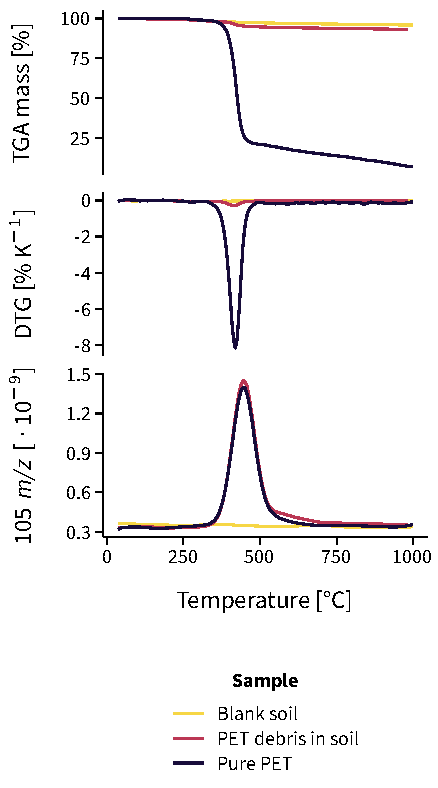
\includegraphics[width=\marginparwidth]{figures/tga-dtg-sample}
	\caption[\Ac{tga} and \ac{dtg} curves of blank soil, pure \ac{pet}, and an exemplary mixture of \ac{pet} debris in soil.]{\Ac{tga} and \ac{dtg} curves and normalized \SI{105}{\mz} ratios of blank soil, pure \ac{pet} (\SI{1.73}{\milli\gram}), and an exemplary mixture of \SI{37.1}{\gram\per\kilo\gram} \ac{pet} debris (\SI{1.74}{\milli\gram}) in soil.}
	\label{fig:tga-dtg-sample}
\end{marginfigure}

The degradation onsets of \ac{pet}, blank soil, and the internal standard \textsc{dl}-cysteine were \SIlist{382;208;205}{\degreeCelsius}, respectively. Figure~\ref{fig:tga-dtg-sample} shows the \ac{tga} curves, \acf{dtg} curves, and \SI{105}{\mz} ratios of blank soil, pure \ac{pet}, plastic dust, and an exemplary \SI{37.1}{\gram\per\kilo\gram} \ac{pet} mixture with soil. The \ac{tga} curve of soil indicated a mass loss of \SI{0.27(3)}{\percent} between \SIrange[range-phrase = { and }]{40}{150}{\degreeCelsius} typically ascribed to soil residual humidity.
Above \SI{208}{\degreeCelsius}, degradation of \ac{som} caused a mass loss of \SI{1.5(1)}{\percent} (calculated until \SI{380}{\degreeCelsius}). The pure \ac{pet} degraded between \SIrange[range-phrase = { and }]{380}{650}{\degreeCelsius} as indicated by a considerable mass loss and accompanied by a peak for \SI{105}{\mz}.
Such a peak was absent in blank soil without any \ac{pet}. As for pure \ac{pet}, soil samples spiked with microplastic \ac{pet} lost its residual humidity between \SIrange[range-phrase = { and }]{40}{150}{\degreeCelsius}.
\Ac{som} degraded above \SI{208}{\degreeCelsius}. The mass loss between \SIrange[range-phrase = { and }]{382}{650}{\degreeCelsius} was attributed to the degradation of \ac{pet}. \textsc{dl}-Cysteine added as internal standard rapidly degraded between \SIrange[range-phrase = { and }]{205}{250}{\degreeCelsius} (Figures~\ref{fig:tga-ms} and \ref{fig:cysteine-tests}).

\begin{figure*}
	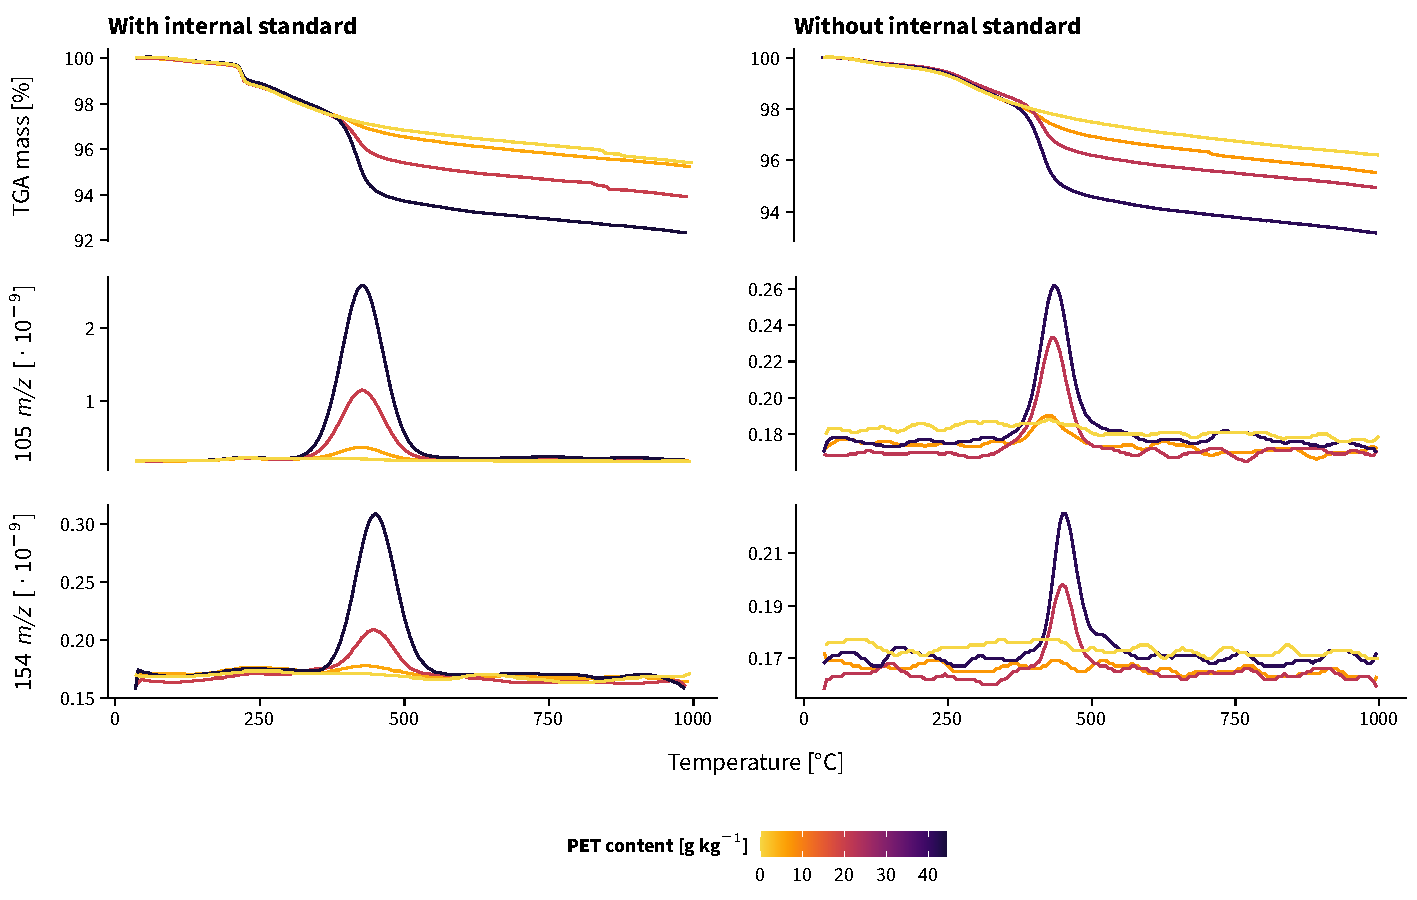
\includegraphics[width=\textwidth]{figures/tga-ms}
	\caption[Exemplary \ac{tga-ms} curves of soil spiked at three different \ac{pet} contents with or without internal standard.]{Exemplary \ac{tga-ms} curves (mass loss, together with \SIlist{105;154}{\mz} ratios) of soil spiked at three different \ac{pet} contents either with or without \textsc{dl}-cysteine as internal standard.}
	\label{fig:tga-ms}
	\forcerectofloat
\end{figure*}

Irrespective of the internal standard, the \SIlist{105;154}{\mz} fragments evolving from pyrolysis of \ac{pet} in soil (Figure~\ref{fig:tga-ms}) corresponded to the mass loss of \ac{pet} on the \ac{tga} curves.
Although these signals have been reported as the most intensive signals occurring during \ac{pet} thermal degradation \citep{DumichenFast2017,DimitrovAnalysis2013}, they cannot be considered absolutely specific for \ac{pet} in soil.
To a certain extent, \SIlist{105;154}{\mz} are also produced during the pyrolysis of \ac{som} \citep{SchultenThermal1999} and other polymers that contain phthalate plasticizers. However, relating \ac{ms} signals to the specific temperature range of \ac{pet} degradation, namely \SIrange{300}{650}{\degreeCelsius}, enabled us to reduce the false positive detection of \ac{pet} degradation products and to correlate them with the nominal \ac{pet} content in soil.
It remains noteworthy that this approach may be restricted to our given setup. Interferences may occur when analyzing other soils containing complex mixtures of different polymers.

Apart from \ac{pet} and \ac{som} degradation products, the sharp mass loss at \SIrange{205}{250}{\degreeCelsius} corresponded to the degradation of \textsc{dl}-cysteine added as internal standard (\SI{33}{\mz}). \textsc{dl}-Cysteine signal intensities were linear in the anticipated concentration range of \SIrange{0.25}{1.78}{\percent} in soil (Figures~\ref{fig:tga-ms} and \ref{fig:cysteine-tests}).

Peaks of \SIlist{105;154}{\mz} ratios integrated within \SIrange{300}{650}{\degreeCelsius} were used for linear calibration curves of \ac{pet} pyrolysis products (Figure~\ref{fig:tga-calibration}). Corresponding \acp{lod}, \acp{loq}, adj. $R^2$s, and \acp{rse} are presented in Table~\ref{tab:tga-calibration}.
Within a linear range of \SIrange{2.5}{40}{\gram\per\kilo\gram} \ac{pet}, the best goodness\-/of\-/fit measures, these were an adj. $R^2$ of \num{0.987} and \iac{rse} of \SI{3.21}{\percent}, were achieved with the \SI{105}{\mz} signal after internal standard addition.
The \ac{lod} and \ac{loq} were \SIlist{0.7;17.2}{\gram\per\kilo\gram} \ac{pet}, respectively. For internal standard-corrected \SI{154}{\mz}, the \ac{lod} was comparable to that of \SI{105}{\mz} as a result of a low background noise.
However, the \ac{ms} signal responded less linearly with increasing \ac{pet} concentrations. Without internal standard, the curve linearity, \acp{lod}, and \acp{loq} were considerably worse.

\begin{figure*}
	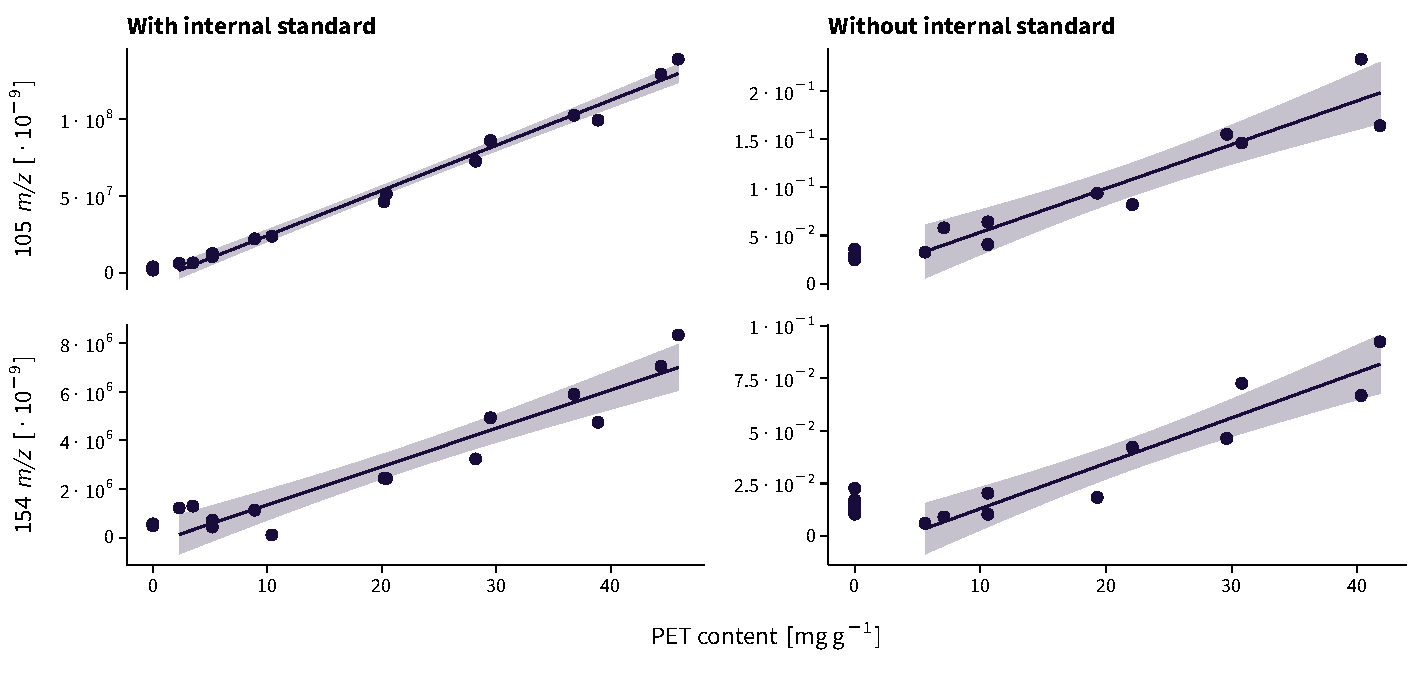
\includegraphics[width=\textwidth]{figures/tga-calibration}
	\caption[\Ac{tga-ms} calibration curves of \ac{pet} in soil.]{\Ac{tga-ms} calibration curves of \ac{pet} (\SIlist{105;154}{\mz}) in soil normalized to the sample mass when no internal standard was added or normalized to \SI{33}{\mz} from the pyrolysis of \textsc{dl}-cysteine as internal standard; shaded bands represent the \SI{95}{\percent} \acs{ci} of the linear model;  calibration parameters are summarized in Table~\protect\ref{tab:tga-calibration}.}
	\label{fig:tga-calibration}
	\forceversofloat
\end{figure*}

\begin{table}[b]
	\centering\footnotesize
	\caption[\Ac{tga-ms} calibration parameters.]{\Ac{tga-ms} calibration parameters; see Figure~\protect\ref{fig:tga-calibration} for calibration curves.}\label{tab:tga-calibration}
	\begin{tabular}{llS[table-format = 1.3]S[table-format = 2.2]S[table-format = 2.1]S[table-format = 3.1]}
		\toprule
		{\si{\mz}} & {Internal standard} & {adj. $R^2$} & {\Acs{rse} [\si{\percent}]} & {\Acs{lod} [\si{\gram\per\kilo\gram}]} & {\Acs{loq} [\si{\gram\per\kilo\gram}]} \\
		\midrule
		105 & no & 0.870 & 12.76 & 2.5 & 510.0 \\
154 & no & 0.888 & 11.75 & 5.8 & 184.0 \\
105 & yes & 0.987 & 3.21 & 0.7 & 17.2 \\
154 & yes & 0.893 & 9.57 & 0.6 & 65.3 \\
		\bottomrule
		\multicolumn{6}{p{.72\textwidth}}{\acs{rse} = \acl{rse} of the slope estimate.} \\
	\end{tabular}
\end{table}

In contrast to our study, \citet{DumichenFast2017} used a common \ac{pe} bag shredded to microplastic particles and an uncharacterized sandy topsoil sampled from an urban area. The authors analyzed various $n$-alkadienes as characteristic products of \ac{pe} pyrolysis via \ac{ted-gc-ms}. They spiked the soil with \SIrange[range-phrase = { to }]{15}{150}{\gram\per\kilo\gram} \ac{pe} concentrations and achieved linear calibration curves of integrated \SI{55}{\mz} signals as a characteristic fragment for eight different $n$-alkadienes with an adj. $R^2$ ranging from \num{0.5395} for 1,11-dodecadiene to \num{0.9958} for 1,15-hexadecadiene. Their highest signal response was observed for 1,13-tetradecadiene, for which an adj. $R^2$ = \num{0.9884} and \iac{loq} of \SI{10}{\gram\per\kilo\gram} \ac{pe} were determined.
\Acp{rse} of slope estimates inferred from the calibration curves by \citet{DumichenAnalysis2015} varied from \SIrange[range-phrase = { to }]{2.97}{12.41}{\percent}. In this respect, our \ac{loq}, adj. $R^2$, and \ac{rse} obtained from \SI{105}{\mz} after internal standard correction (\SI{17.2}{\gram\per\kilo\gram} \ac{pet}) were generally comparable with those by \citet{DumichenAnalysis2015}.
Small differences in adj. $R^2$s, \acp{lod}, and \acp{loq} are probably due to use of a different soil and polymer. In addition to that, we tried to mimic a potential environmentally relevant \ac{pet} sample with the dust that originated from shredding of recycled \ac{pet} bottles.
Although checked by \ac{dsc}, recycled \ac{pet} dust may contain impurities from different polymer or paper microparticles.
When pyrolyzed, such impurities may interfere with \num{105} or \SI{154}{\mz} signals produced by pure \ac{pet}.
Together with \ac{pet} concentrations up to \num{6} times lower than the \ac{pe} contents used by \citet{DumichenAnalysis2015}, a slightly higher variation in detector responses and, with that, a reduced goodness of fit of the calibration curves are deemed plausible. One option to further reduce detector variation could be to recalibrate the \ac{sem} voltage after every sample run, which is however, not practical for routine analyses. This is why we normalized the obtained signals to an internal standard, which increased the linearity of the calibration curves (Figure~\ref{fig:tga-calibration}).
Moreover, \ac{tga-ms} has so far mostly been used to analyze pure chemicals with known stoichiometry of decomposition reactions and low-molecular-weight pyrolysis products \citep{HotovaQuantitative2016}. Reactions of pyrolysis products potentially occurring in the heated capillary may therefore be another reason for less sensitive signal responses, which we assessed with regular capillary tests.

\subsection{Transfer Capillary Control Experiments}

Series of cleaning runs confirmed that no signal of \SI{105}{\mz}\sidenote{As the stronger of the \si{\mz} ratios analyzed.} was detected in runs following soil analysis. Figure~\ref{fig:tga-capillary-checks} shows worst case scenarios, this is cleaning run and oxalate run after the most concentrated spiked samples, where the probability of capillary blocking was the highest, both with and without \textsc{dl}-cysteine as internal standard.
The results are in comparison with the best case scenarios, namely cleaning run and oxalate run after the least concentrated spiked samples and the \SI{105}{\mz} signals of both least concentrated \ac{pet} samples.
Note that the baselines of the least spiked samples (\SI{2}{\gram\per\kilo\gram} \ac{pet}) vary in comparison to cleaning runs, because the cleaning runs were performed in synthetic air.

\begin{figure*}
	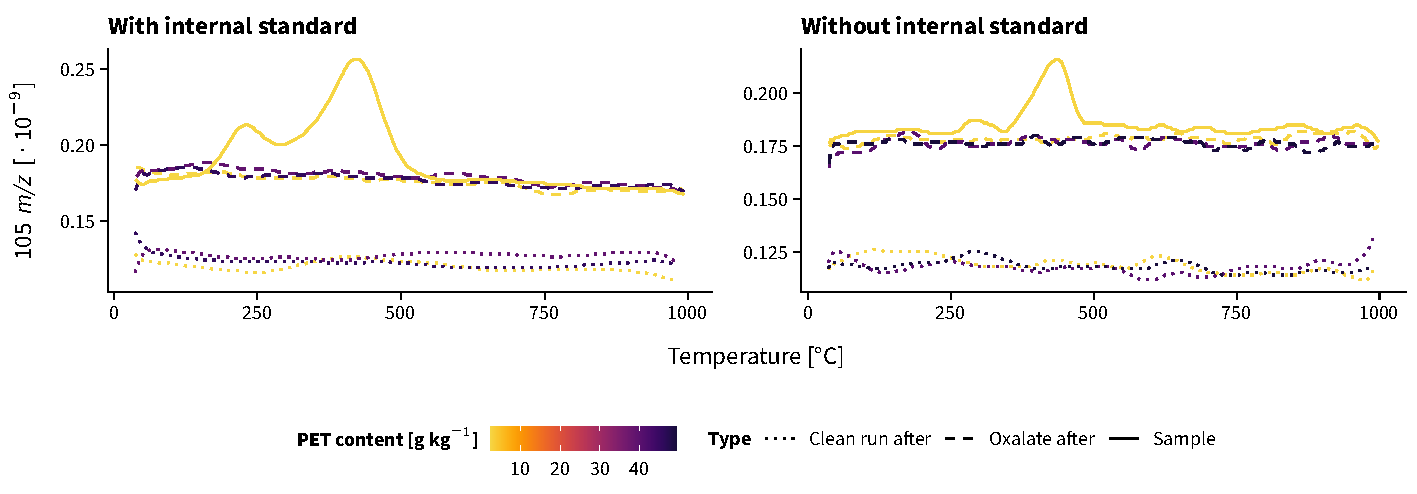
\includegraphics[width=\textwidth]{figures/tga-capillary-checks}
	\caption[\SI{105}{\mz} ratios of selected cleaning runs and calcium oxalate hydrate pyrolyses after measuring a highly concentrated \ac{pet} sample and the least concentrated sample with or without internal standard.]{\SI{105}{\mz} ratios of selected cleaning runs and calcium oxalate hydrate pyrolyses after measuring a highly concentrated \ac{pet} sample (\SI{>40}{\gram\per\kilo\gram}, worst case) and the least concentrated sample (\SI{2}{\gram\per\kilo\gram}, best case) in comparison to the same signal of the lowest spiked soil sample either with or without \textsc{dl}-cysteine as internal standard.}
	\label{fig:tga-capillary-checks}
	\forcerectofloat
\end{figure*}

The \acp{snr} of \SI{105}{\mz} without internal standard correction ranged from \numrange[range-phrase = { to }]{51}{96} with respect to cleaning runs and from \numrange[range-phrase = { to }]{90}{128} when based on oxalate pyrolysis runs.
With internal standard added, the \acp{snr} were \numrange{26}{354} and \numrange{45}{315} for cleaning runs and oxalate pyrolysis runs, respectively. Figure~\ref{fig:tga-capillary-checks} shows that during cleaning runs and oxalate pyrolysis, no interfering \SI{105}{\mz} signals were found. With \textsc{dl}-cysteine added as internal standard, we found a small shoulder peak between \SIrange[range-phrase = { and }]{170}{300}{\degreeCelsius} probably originating from 2-methylthiazolidine (\SI{103}{\mz}), a byproduct of cysteine pyrolysis \citep{FujimakiPyrolysis1969}.
The \SI{103}{\mz} fragment may become visible due to the presence of heavier isotopologues and insufficient mass resolution of the \ac{tga-ms}. An additional indication for a working capillary was provided by the pressure measurements in the capillary performed before each experiment. The capillary pressure was within the normal range of \SIrange[range-phrase = { to }]{2e-5}{8e-6}{\milli\bar}.
Capillary pressures below \SI{8e-6}{\milli\bar} would indicate a blocked capillary. Pressures above \SI{2e-5}{\milli\bar} may result from a break in the capillary (Figures~\ref{fig:control-measurements} and \ref{fig:tga-capillary-pressure}). Therefore, it was assumed that the capillary had not become blocked during the analyses. Capillary conditions were further checked by observing the peaks of \ch{H2O} (\SI{18}{\mz}), \ch{CO} (\SI{28}{\mz}), and \ch{CO2} (\SI{44}{\mz}) resulting from stoichiometric calcium oxalate hydrate pyrolysis.
For quantitative determination of pyrolysis products of plastic materials, we recommend introducing this capillary checking procedure
in between sample measurements. In our case, the variation of obtained \ch{H2O}, \ch{CO}, and \ch{CO2} signals of the control calcium oxalate runs was within the common limits of the \ac{tga-ms} device used \citep{NetzschGeratebauMS2010}.

\section{Conclusions}

With this study, we showed for the first time the suitability of \ac{tga-ms} for the quantitative analysis of \ac{pet} plastic debris in a standard loamy sand with \SI{1.6(2)}{\percent} \ac{Corg}. We considerably improved signal sensitivities and linearity by using \textsc{dl}-cysteine as an internal standard. This broadens the application of \ac{tga-ms}, bringing new insight into the emerging field of microplastics research in soil science. Follow-up studies will need to show whether a similar analytical setup could be extended to standard soils with different \ac{Corg} contents and real soil samples polluted with \ac{pet} debris. However, high \ac{Corg} contents, for instance from applied sewage sludge, or contamination with other polymers would probably interfere with \ac{pet} or internal standard pyrolysis products. Such challenges could be further addressed using chemically assisted pyrolysis or deconvolution techniques combined with a simple sample preparation method to reduce noise from the sample matrix. This would also enable us to further reduce \acp{loq} to approach environmentally relevant \ac{pet} contents.

Although recently published methods using \ac{ted-gc-ms} \citep{DumichenAnalysis2015}, \ac{py-gc-ms} \citep{FischerSimultaneous2017}, and \ac{lc-ms} \citep{WangSimple2017} produced lower or equal \acp{loq} than this study, \ac{tga-ms} measurements are generally cheaper and require only a minimal sample preparation effort. In addition, \ac{tga-ms} can be used with various heating rates and sample amounts up to \SI{1}{\gram} \citep{JakabThermal2003}, which will be needed to account for the heterogeneity of soil samples.
We therefore consider \ac{tga-ms} a valuable complement to existing analytical methods in terms of serving as a first assessment tool for plastic debris in soil in order to further elucidate if agricultural soils are a potential sink for plastic debris.
